\documentclass[../main.tex]{subfiles}
\begin{document}

\subsection{Categorical}
\label{sec:categorical}
Categorical data, including vectors of categorical observations, can be represented as sets; researchers then query set cardinality, membership, and intersections \cite{agresti_categorical_2011,schneider_set-theoretic_2012}. In exploring these intersections, the question arises of which categories appear in conjunction with each other and if any one category is the driving force underlying the frequency of other categories. For example, in frequent item set detection, the task is to figure out the minimum set of items that can be used to predict the occurrence of other items in the set \cite{leskovec_mining_2014,Srikant:1997:MAR:3001392.3001404}. By representing categorical variables as sets, we can exploit methods of set visualization to explore dependencies amongst categorical variables.

\subsubsection{Cross Table}
\label{sec:crosstab}
\begin{figure}[H]
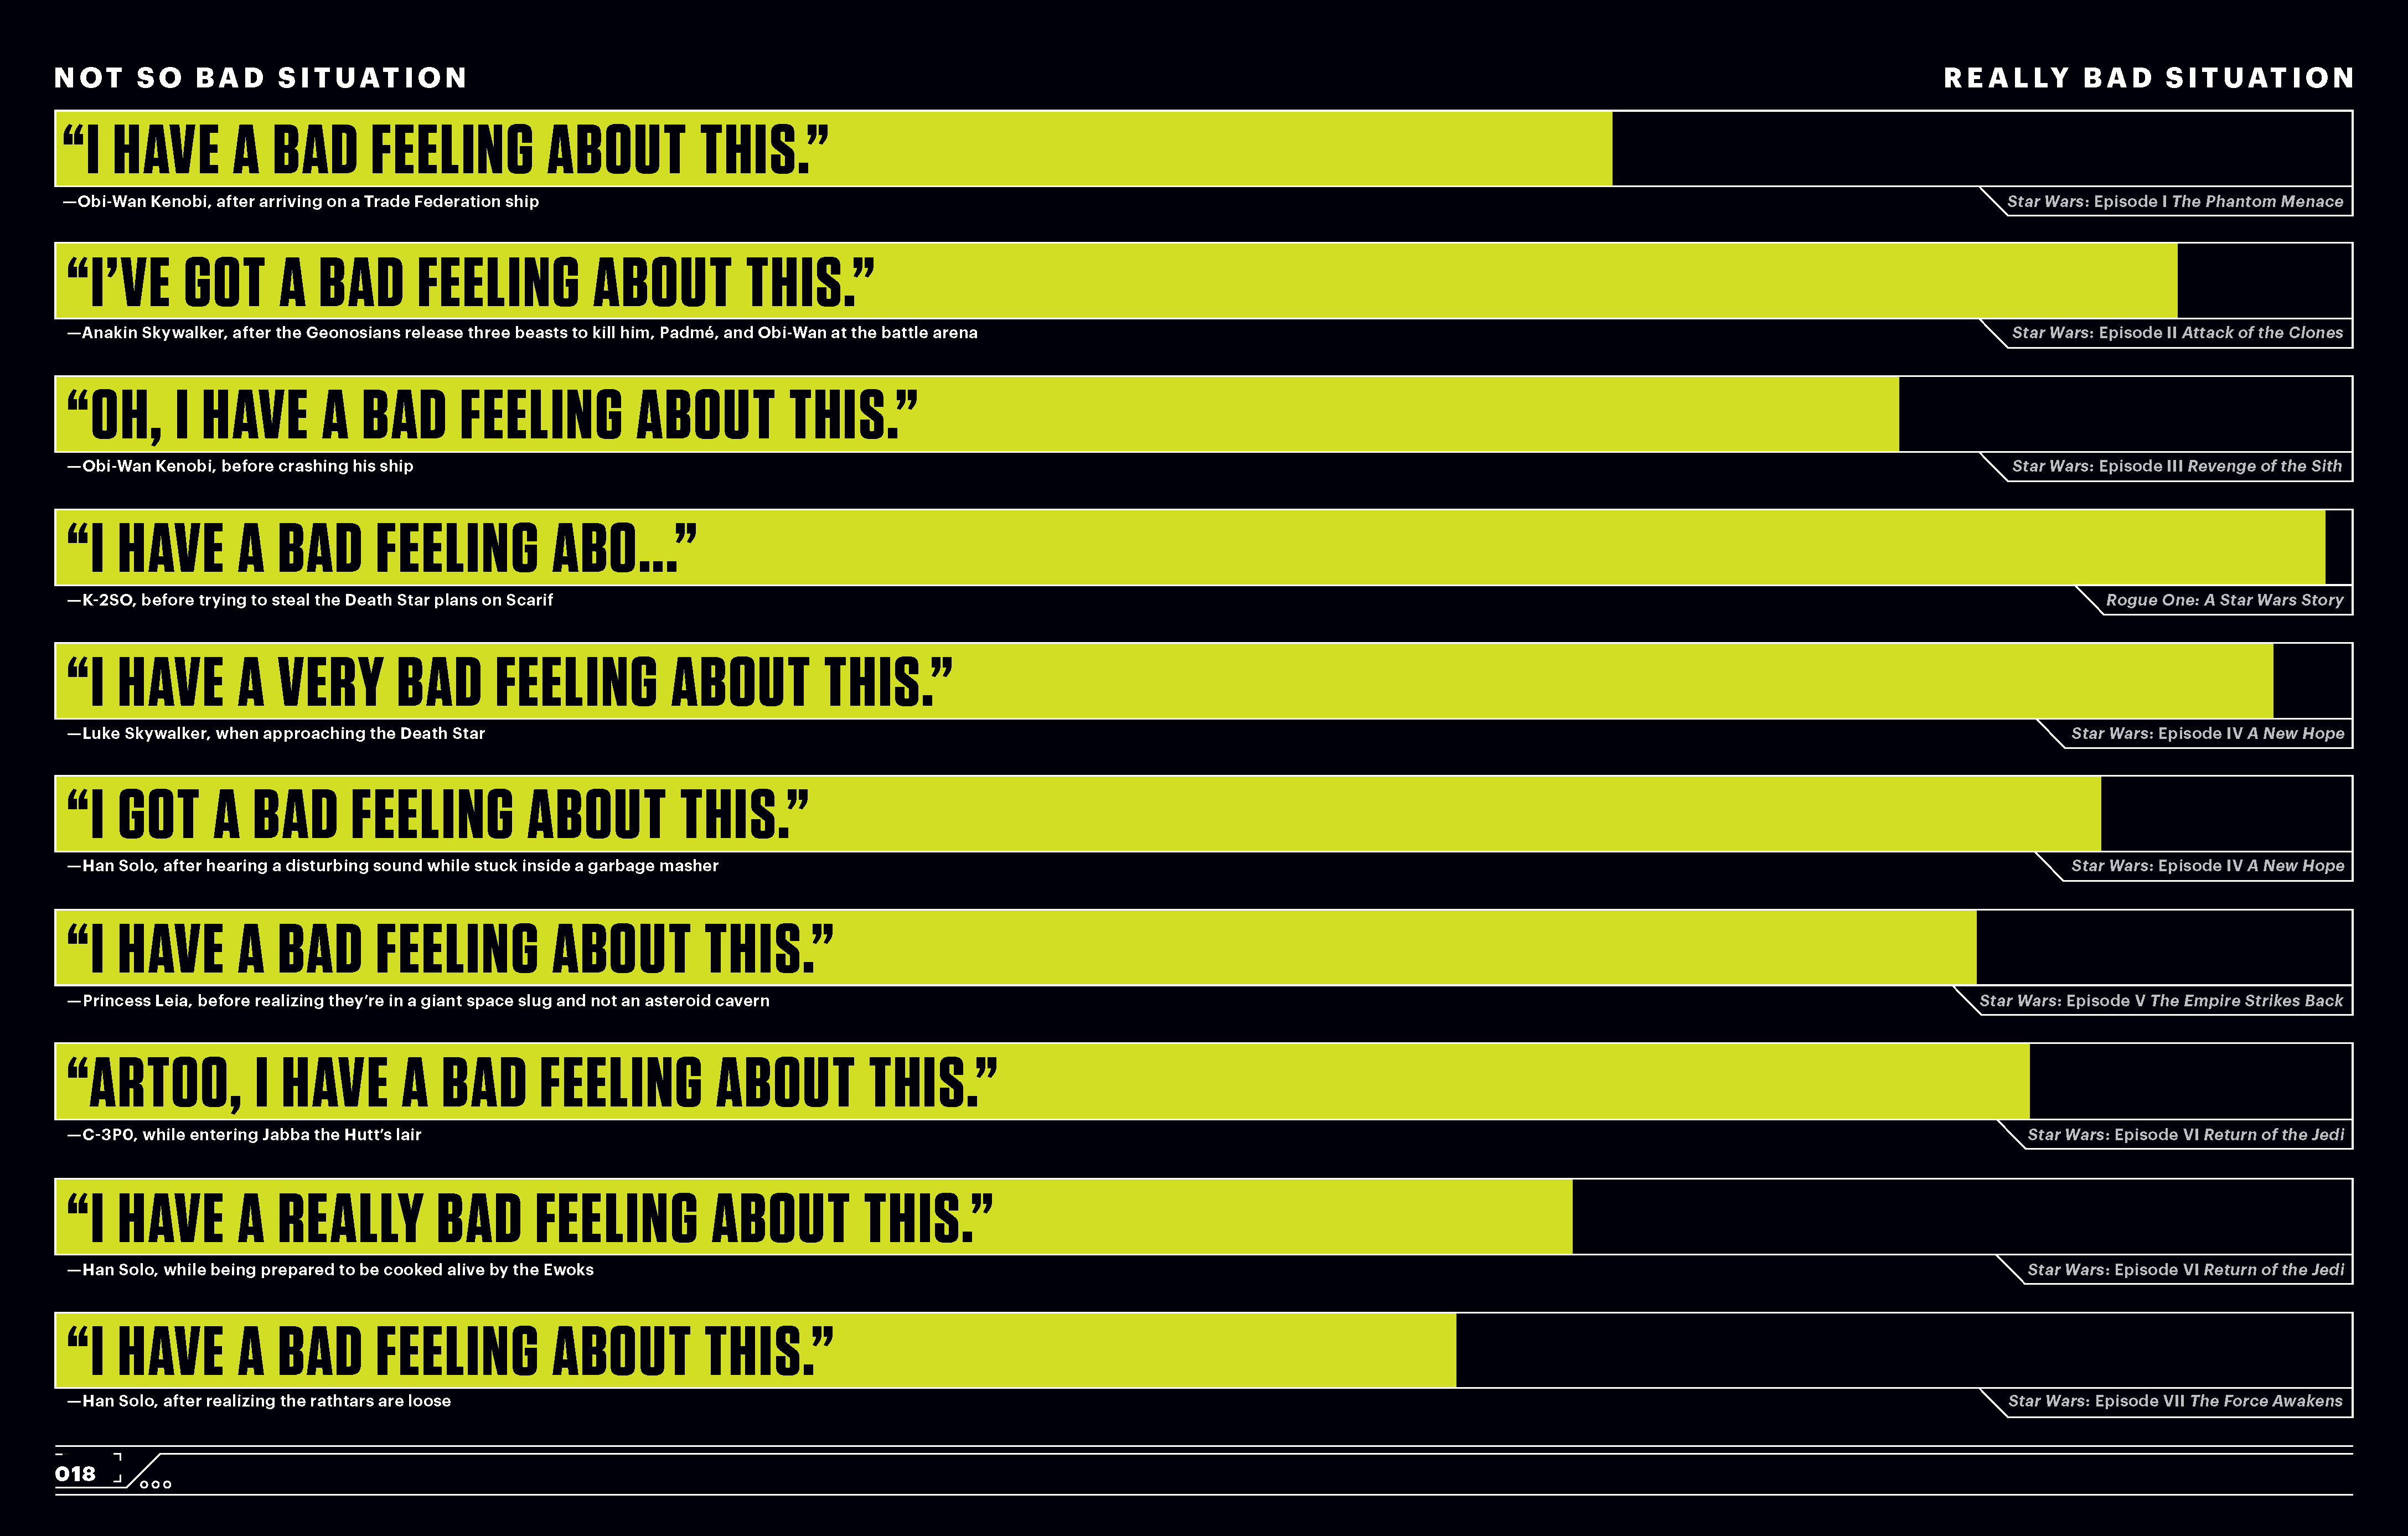
\includegraphics[width=1\textwidth]{swsg.png}
\caption{Graphic designer Tim Leong visualizes a cross table of a phrase against the severity of the situation in which it was said. Because the situations are ordered chronologically, this illustration shows that the most severe situations occur in the middle of the Star Wars' timeline. Chart is from \textit{Star Wars Super Graphic} \cite{leong_star_2017}}
\label{fig:starwars}
\end{figure}

One of the most common approaches for understanding relationships between categorical variables is to aggregate a function applied to the product of two or more sets; this computation is called a cross table \cite{goodman_measures_1991}. Figure~\ref{fig:starwars} is a visual example of a cross table where the sets are a phrase spoken by a character in a Star Wars film and the severity of the situation in which the phrase is spoken \cite{leong_star_2017}. Designer Tim Leong structures the visualization such that the phrases are chronologically ordered with respect to the Star Wars' timeline and he lines up the phrases such that variations are readily apparent. He then encodes the probability of danger as the height of the yellow bar such that the more dangerous, the more it encroaches on the \textit{Really Bad Situation} side of the visualization. Each phrase is a set with one element (the phrase), and the cross tabulation is the likelihood that the speaker is in a dangerous situation. Because the phrases are ordered in temporal order, Leong's visualization suggests that there is a higher likelihood of bad events happening near the middle of the timeline, indicating that severity of situational badness and the type of phrasing used could be conditionally dependent on the location of the event- in the story arc. Leong effectively uses a cross table to visualize a small number of groups (phrases) and a very small number of variables (phrases, situations). Cross-tabulations shine when there are a few variables and a small number of groups, but get very unwieldy as the size of the set product grows. 

\begin{figure}[H]
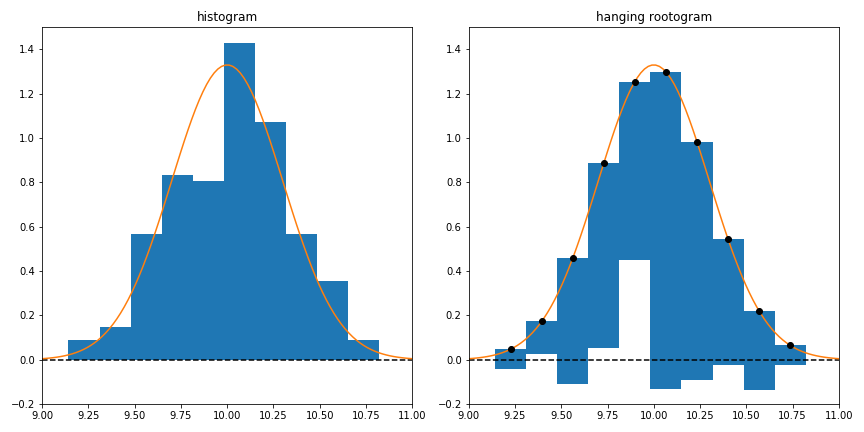
\includegraphics[width=1\textwidth]{hanging_rootgram.png}
\caption{The hanging rootogram shifts the histogram bars up so that they intersect with the expected values of the density estimator. This means that deviations between the expected and observed frequencies can be measured as the distance between the bottom of the rectangle and horizontal line at x=0.}
\label{fig:hanging_rootogram}
\end{figure}
 While a simple table is encouraged for a small number of variables or categories \cite{munzner_visualization_2014}), bar graphs and histograms \cite{ioannidis_history_2003-1, friendly_brief_2006} are more appropriate when the variable has a large number of unique categories or the dataset has a large number of variables. Variations on histograms  include the hanging rootogram shown in figure~\ref{fig:hanging_rootogram} and other distribution oriented plots \cite{tukey_exploratory_1977, friendly_visualizing_2000}. While conditional relationships can be visualized using other categorical visualizations such as fourfold displays, mosaic displays, and logit regression models, these plots are somewhat limited to 3 categorical variables \cite{friendly_visualizing_2000}. For datasets with more complex categorical relationships, we can look to set oriented visualization tools 
   
 \subsubsection{Set Intersection}
 \label{sec:setintersection}
\begin{figure}[H]
  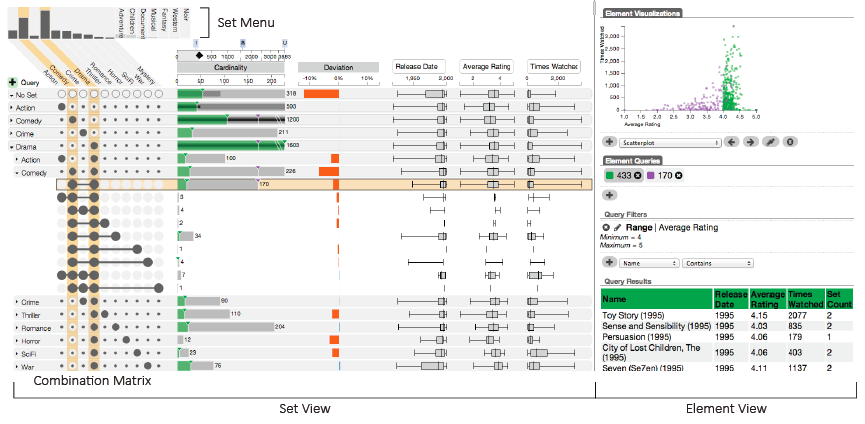
\includegraphics[width=\textwidth]{upsetfig1}
   \caption{UpSet dashboard displaying the relationships between a movie's genre and its release date, ratings, and popularity. The left panel of the dashboard lets the user query the database for all movies in a selected genre. It then shows which other genres these movies belong to. The middle panel shows the distribution of release dates, ratings, and popularity of the movies in each intersecting set of genres. The right panel lists the individual movies in one of these intersecting sets and plots their quantitative attributes as scatter plot. This combined visualization tool allows a user to see if quantitative attributes like ratings or popularity are conditionally dependent on the genre. This figure comes from \textit{UpSet: Visualization of Intersecting Sets} \cite{lex_upset_2014}}
   \label{fig:upsetfig}
\end{figure}

The UpSet tool is designed to display a large number of set intersections, frequency information about set membership, and information about the distribution of quantitative attributes of elements in a set \cite{lex_upset_2014}. As shown in figure~\ref{fig:upsetfig}, the UpSet tool provides linked set and element views so that users can get a top level view of the characteristics of a genre of movies and also information about the movies in that genre. The set view on the left panel of the dashboard lets users select a genre and then displays information about how many movies are in that genre and what other genres those movies belong to. The middle panel shows the distribution of the release dates, average ratings, and popularity of the movies in each of the sets shown on the right side. The right panel element view displays the movies in the selected genre and the scatter plot shows each movie's ratings and popularity. The UpSet tool provides a window into conditional dependency because a user can see if attributes of the movies in a genre, such as average movie rating and release date, are conditionally dependent on genre. Users can select a genre (e.g. comedy) and look at how the attributes of the movies in that set distribute and then compare those results against the distributions of other genres. While the UpSet tool can handle data that is too complex for cross tables (\ref{sec:crosstab}), it can not preserve structure and is limited to showing intersections of sets of one variable type (e.g. only genres) and a low number of quantitative variables.  

\end{document}


